\section{Deutsch und Kommunikation}


%%% Anfang: tl;dr
\subsection{tl;dr - Zusammenfassung der Zusammenfassung}
%%% Ende: tl;dr

%%% Anfang: Lernen
\subsection{Lernen}


%%% Anfang: Lernen > Physiologie
\subsubsection{Physiologische Voraussetzungen des Lernerfolges}

\paragraph{Aufbau des Gehirns}~\\
\\
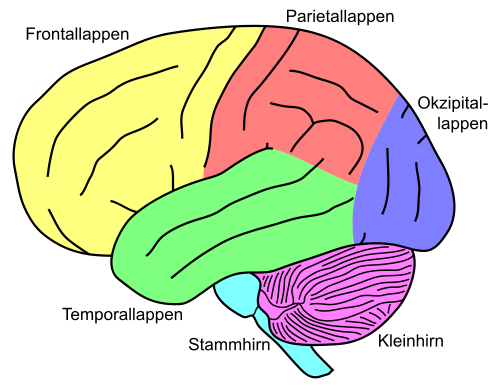
\includegraphics[scale=0.7]{pictures/dko-pic/dko-gehirnaufbau.png}~\\
\\
Der {\bf Parietallappen} (auch Scheitellappen genannt) ist für die Integration sensorischer Informationen zuständig. Im vorderen Teil wird die haptische Wahrnehmung (Berührung, Druck, Vibration, Temperatur und teilweise auch Schmerz) verarbeitet. Der obere Teil hingegen ist zuständig für die visuelle Bewegungssteuerung und die Erkennung von Reizen im betrachterbezogenen Raum. Somit ermöglicht dieser Teil des Gehirns die räumliche Aufmerksamkeit. Im unteren Teil des Parietallappens finden das räumliche Denken und \ql quasi-räumliche\qr\ Prozesse wie Rechnen und Lesen statt.\\
\\
Im {\bf Okzipitallappen} (auch Hinterhauptlappen genannt), befinden sich die primäre und die sekundäre Sehrinde. In der primären Sehrinde werden die Signale der Netzhaut verarbeitet. Die sekundäre Sehrinde dient dem Gehirn als Assoziationszentrum. Sie stellt die Verarbeiteten Muster aus der primären Sehrinde bekannten Sinneseindrücken gegenüber, interpretiert und erkennt sie. Zudem stellt sie eine Verknüpfung mit anderen Rindenarealen des Großhirns dar.\\
\\
Im {\bf Kleinhirn} wird die Feinsteuerung der Motorik vorgenommen. Beim implizierten Lernen (unbewusste oder spielerische Aneignung von Fertigkeiten und Wissen beim Ausüben einer Tätigkeit) spielt es eine große Rolle, da es die automatisierten Tätigkeiten speichert.\\
\\
Das {\bf Stammhirn} besteht aus dem {\it verlängerten Rückenmark}, der {\it Brücke} und dem {\it Mittelhirn}. Das verlängerte Rückenmark hat eine Schlüsselposition im Nervensystem des Körpers. Alle Nervenbahnen, die das Gehirn mit dem Körper verbinden, fließen durch das verlängerte Rückenmark. Zusätzlich ist es für die Kontrolle des Blutkreis und der Atmung zuständig. So befinden sich zum Beispiel die Rezeptoren zur Steuerung des Atemreflexes dort. Weitere wichtige Reflexe, die aus dem verlängerten Rückenmark gesteuert werden sind Nies-, Husten-, Schluck- und Saugreflex sowie das Erbrechen. \\
Die Brücke dient als Durchgangsstation für alle Nervenfasern zwischen den vorderen und dahinterliegenden Abschnitten des Zentralnervensystems sowie als Umschaltstation zwischen dem Großhirn und dem Kleinhirn.\\
Das Mittelhirn steuert die Augenmuskulatur und leitet die Erregungen sensibler Nerven an das Großhirn weiter.\\
\\
Der {\bf Temporallappen} (Schläfenlappen) ist für die Verarbeitung der akustischen Signale zuständig. In ihm befindet sich auch das {\it sensorische Sprachzentrum}, welches für das Sprachverständnis wichtig ist. Weiterhin wird hier auch das visuelle Arbeitsgedächtnis lokalisiert, was der kurzen Speicherung von aktuellen Wahrnehmungen dient. Auch der Vergleich mit den nächstfolgenden Wahrnehmungsinhalten und das Erkennen von komplexen nichträumlichen auditorischen und visuellen Reizen (z.B. das Erkennen von Gesichtern) findet im Temporallappen statt.\\
\\
Im {\bf Stirnhirn} findet die Steuerung der Bewegungen sowie das Auswählen von Bedingungen für diese Bewegungen statt. Die kognitiven Prozesse werden hier reguliert um eine situationsgerechte Ausführung von Handlungen sicherzustellen. Im Stirnhirn befindet sich auch das motorische Sprachzentrum, welches die Motorik zur Produktion der Sprache steuert.\\
\paragraph{Das Nervensystem}~\\
\\
Das menschliche Nervensystem besteht aus hochspezialisierten einzelnen Zellen({\it Neuronen}). Diese Zellen können sich jedoch nicht mehr teilen, weshalb Verletzungen im Nervensystem nicht heilen können. Die Zellen sind untereinander verbunden (ein neugeborenes Kind hat ca. 50 Billionen Verbindungen zwischen den Nervenzellen) und senden Signale aus, sobald die Summe der Eingangssignale einen Bestimmten Schwellenwert überschreitet. Eine Einteilung des Nervensystems kann nach verschiedenen Kriterien erfolgen. Für den Lernprozess ist allerdings die Klassifizierung in das vegetative und das somatische Nervensystem am wichtigsten.\\
Das {\bf vegetative Nervensystem} (Autonomes Nervensystem) ist der willentlichen Kontrolle weitestgehend entzogen. Es dient der Steuerung der inneren Organe.\\
Das {\bf somatische Nervensystem} (willkürliches oder animalisches Nervensystem) dient der Wahrnehmung von Umweltreizen und Reizen aus dem Körperinneren sowie der Steuerung der dem Bewusstsein und dem Willen unterworfenen Vorgängen. Dies impliziert bewusste ebenso wie willkürliche Bewegungen.

%%% Anfang: Lernen > Typen
\subsubsection{Welche Lerntypen gibt es?}

\paragraph{Visueller Lerntyp}~\\
\paragraph{Haptischer Lerntyp}~\\
\paragraph{Auditiver Lerntyp}~\\
\paragraph{Kommunikativer Lerntyp}~\\

%%% Anfang: Lernen > Methoden
\subsubsection{Lernmethoden}

\paragraph{10 Lernmethoden}~\\
\begin{itemize}
	\item Notizen
	\item Markieren
	\item Mindmap
	\item Case Studies
	\item Karteikarten
\end{itemize}

%%% Anfang: Lernen > Faktoren
\subsubsection{Äußere Einflussfaktoren auf den Lernerfolg}
\paragraph{Einfluss der direkten Umgebung}~\\
\paragraph{Einfluss des sozialen Umfeldes}~\\
\paragraph{Einfluss der Ernährung}~\\
Das Gehirn kann im Gegensatz zum Rest des Körpers nur mit Glukose umgehen. Generell gilt, je höher der Glukosespiegel ist, desto besser können wir uns konzentrieren und desto besser ist unsere geistige Leistungsfähigkeit. Jedoch gibt es ein oberes Limit, ab dem der Körper vermehrt Insulin produziert, welches den Glukosespiegel rapide sinken lässt. Es folgen Müdigkeit, Konzentrationsstörungen und generell eine geringere Leistungsfähigkeit. Statt stark zuckerhaltige Lebensmittel zu verzehren, sollten also Lebensmitteln mit einem hohen Anteil an komplexen Kohlenhydraten bevorzugt werden, damit der Glukosespiegel nicht zu schnell steigt und über einen längeren Zeitraum konstant bleibt.
Konzentrationsschwäche kann aber auch dann auftreten, wenn dem Körper bestimmte Mineralien fehlen wie bspw. Eisen. Für optimale Leistungsfähigkeit sollte auf eine gesunde Ernährung geachtet werden.
\paragraph{Einfluss von Drogen}~\\

%%% Ende: Lernen
%%%%%%%%%%%%%%%%%%%%%%%%%%%%%%%%%%%%%%%%%%%%%%%%%%%%%%%%%%%%%%%%%%%%%%%%%%%%%%%%